\documentclass[tikz, border=10pt]{standalone}
\usepackage{pgfplots}
\pgfplotsset{compat=1.18}

\begin{document}
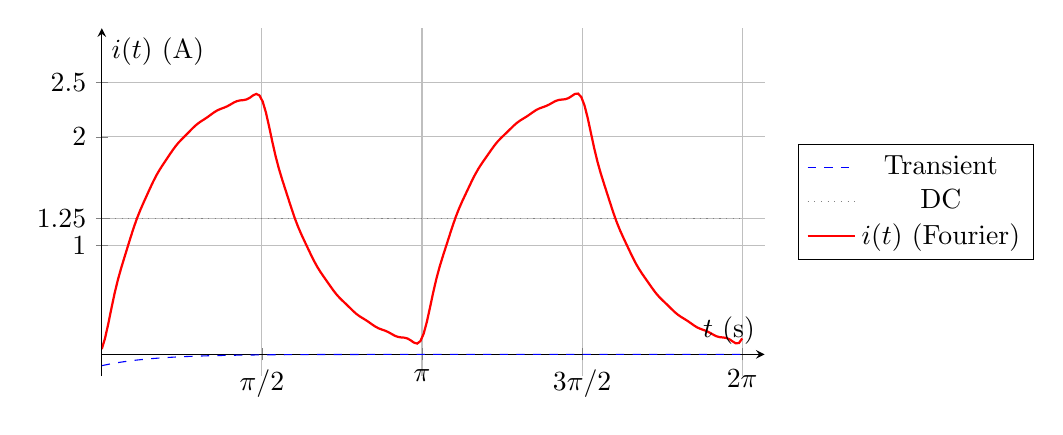
\begin{tikzpicture}
    \begin{axis}[
        axis lines = middle,
        xlabel = {$t$ (s)},
        ylabel = {$i(t)$ (A)},
        xmin = 0, xmax = 6.5,
        ymin = -0.2, ymax = 3.0,
        xtick = {0, 1.57, 3.14, 4.71, 6.28},
        xticklabels = {0, $\pi/2$, $\pi$, $3\pi/2$, $2\pi$},
        ytick = {0, 1, 1.25, 2, 2.5},
        grid = both,
        width=10cm, height=6cm,
        legend style={at={(1.05, 0.5)}, anchor=west},
        samples=200,
        domain=0:6.28
    ]
    
    % Transient Term
    \addplot[blue, dashed, domain=0:6.28] {-0.104*exp(-2*x)};
    \addlegendentry{Transient}
    
    % DC Term
    \addplot[gray, dotted, domain=0:6.28] {1.25};
    \addlegendentry{DC}

    % Fourier Series approximation (Sum of 8 terms)
    \addplot[red, thick] {
        -0.104*exp(-2*x) + 1.25 + (5/pi) * (
            (sin(deg(2*1*x))/(1*(1+1))) - (cos(deg(2*1*x))/(1+1)) +
            (sin(deg(2*3*x))/(3*(1+9))) - (cos(deg(2*3*x))/(1+9)) +
            (sin(deg(2*5*x))/(5*(1+25))) - (cos(deg(2*5*x))/(1+25)) +
            (sin(deg(2*7*x))/(7*(1+49))) - (cos(deg(2*7*x))/(1+49)) +
            (sin(deg(2*9*x))/(9*(1+81))) - (cos(deg(2*9*x))/(1+81)) +
            (sin(deg(2*11*x))/(11*(1+121))) - (cos(deg(2*11*x))/(1+121)) +
            (sin(deg(2*13*x))/(13*(1+169))) - (cos(deg(2*13*x))/(1+169)) +
            (sin(deg(2*15*x))/(15*(1+225))) - (cos(deg(2*15*x))/(1+225))
        )
    };
    \addlegendentry{$i(t)$ (Fourier)}

    \end{axis}
\end{tikzpicture}
\end{document}
